\documentclass{article}

\usepackage[hangul]{kotex}
\usepackage{amsmath}
\usepackage{tikz}
\usepackage{minted}
\usepackage{geometry}
\usepackage{enumitem}
\usepackage{multicol}
\usepackage[linguistics]{forest}
\usepackage{algorithm}
\usepackage{algpseudocode}
\usepackage{hyperref}
\usepackage{caption}

\hypersetup{
  colorlinks = false, %Colours links instead of ugly boxes
  urlcolor = blue, %Colour for external hyperlinks
  linkcolor = black, %Colour of internal links
  citecolor = red %Colour of citations
}

\geometry{
  a4paper,
  left=2.7cm,
  right=2.7cm,
  top=2.7cm,
  bottom=2.7cm,
}

\setmonohangulfont{Fira Code}[AutoFakeSlant]
\setmonofont{Fira Code}[AutoFakeSlant]

\title{프로그래밍과 문제해결 \\ Assignment \#4}
\author{무은재학부 박재원 (2024****)}
\date{\today}

\begin{document}

\begin{titlepage}
	\centering
	{\huge CSED101 프로그래밍과 문제해결\par}
	\vspace{0.5cm}
	{\LARGE Assignment \#4\par}
	\vspace{0.5cm}
	{\large \today\par}
	\vfill
  
  \begin{multicols}{2}
    \vphantom{}
    \columnbreak
  {
    \Large 
    \begin{description}[nosep, align=right, labelwidth=\widthof{00000000000000000}]
      \item[학과] 무은재학부
      \item[학번] 2024****
      \item[이름] 박재원
      \item[POVIS ID] ****
    \end{description}
  }
  \end{multicols}

  \vspace{1cm}


  \begin{quote}
    명예서약 (Honor code)

    ``나는 이 프로그래밍 과제를 다른 사람의 부적절한 도움 없이 완수하였습니다.''
  \end{quote}

\end{titlepage}

\tableofcontents

\section{개요}

본 과제는 Connect Four 게임을 구현하는 것이다. Python과 Tkinter를 활용하여 GUI로 구현해야 하며,
두 플레이어가 하나의 컴퓨터로 플레이 할 수 있도록 구현해야 한다. 

Connect Four는 두 플레이어가 번갈아 가며 본인 색의 공을 직사각형 판에 떨어뜨려,
본인의 공 4개를 직선으로 연속해서 연결한 플레이어가 승리하는 게임이다.

\section{설계}

\subsection{구조도}

프로그램의 전체 구조도는 그림 \ref{fig:structurechart}와 같다. 

Info 클래스는 게임 화면 상단의 현재 플레이어 정보를 담당하며, Board는 하단의 게임판 및 사용자 입력 정보를 담당한다.
Ball 클래스는 게임판의 공 하나를 담당하여 공 표시 및 이동 애니메이션을 담당한다.

\begin{description}
  \item[입력부] 마우스 이동(현재 선택된 열 판단), 마우스 클릭(착수)
  \item[처리부] 착수 처리, 승부 결정/무승부 판단 등
  \item[출력부] 플레이어 정보, 게임판 및 착수된 공, 사용자 입력 정보 GUI로 출력, 승부 결과 window 표시 등
\end{description}

\begin{figure}
  \begin{center}
    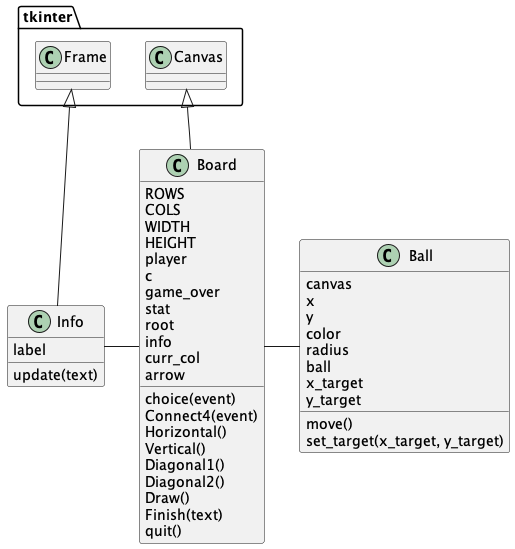
\includegraphics[width=8cm]{assets/structure_chart.png}
    \caption{본 프로그램의 전체 구조도}
    \label{fig:structurechart}
  \end{center}
\end{figure}

\subsection{알고리즘}
프로그램의 알고리즘을 의사코드로 나타내면 알고리즘 \ref{alg:all}\과 같다.

\begin{algorithm}
  \caption{본 프로그램 주요 부분의 의사 코드} \label{alg:all}
  \begin{algorithmic}
    \State 위젯 인스턴스 생성 및 화면 구성 요소 출력
    \While {}
      \If {마우스 이동}
        \State 선택된\_열 $\gets$ (마우스 x 좌표) $\div$ (한 cell 가로 길이) 의 몫
        \State 사용자 입력 정보 갱신
      \EndIf
      \If {마우스 클릭}
        \If {선택된 열 맨 꼭대기(index 0)에 공이 있다}
          \State 이벤트 무시하기
        \EndIf
        \State 선택된\_행 $\gets$ 선택된 열의 항목 중 값이 white면서 가장 아래에 있는(index가 가장 큰) 행
        \State 공 인스턴스 생성 및 선택된 열 및 행으로 이동
        \State stat 업데이트
        \If {연속된 공 4개가 존재한다}
          \State 마지막으로 착수한 유저 승리 메시지 출력 및 게임 오버 창 생성 및 프로그램 종료
        \EndIf
        \If {모든 게임판이 공으로 찼다}
          \State 무승부 메시지 출력 및 게임 오버 창 생성 및 프로그램 종료
        \EndIf
        \State 사용자 턴 전환 및 현재 턴 출력
      \EndIf
    \EndWhile
  \end{algorithmic}
\end{algorithm}

\section{실행 방법 및 예제}

본 과제는 MacOS\footnote{특정 OS에 종속적인 기능을 사용하지 않으므로 다른 운영체제에서도 정상 작동하리라 예상된다.}, CPython 3.12.2에서 작성 및 테스트되었다.

본 과제를 실행하려면 다음과 같이 assn4.py 파이썬 파일을 실행하면 된다.
프로그램을 실행하면 GUI window가 나타난다. 해당 window와 마우스 이동 및 클릭으로 상호작용하면서 프로그램을 사용할 수 있다.
\begin{minted}[]{bash}
  ls
  # assn4.py
  python assn4.py
\end{minted}

실제 프로그램 실행 모습은 그림 \ref{img:1} $\sim$ \ref{img:4}와 같다.

\begin{figure}
  \begin{center}
    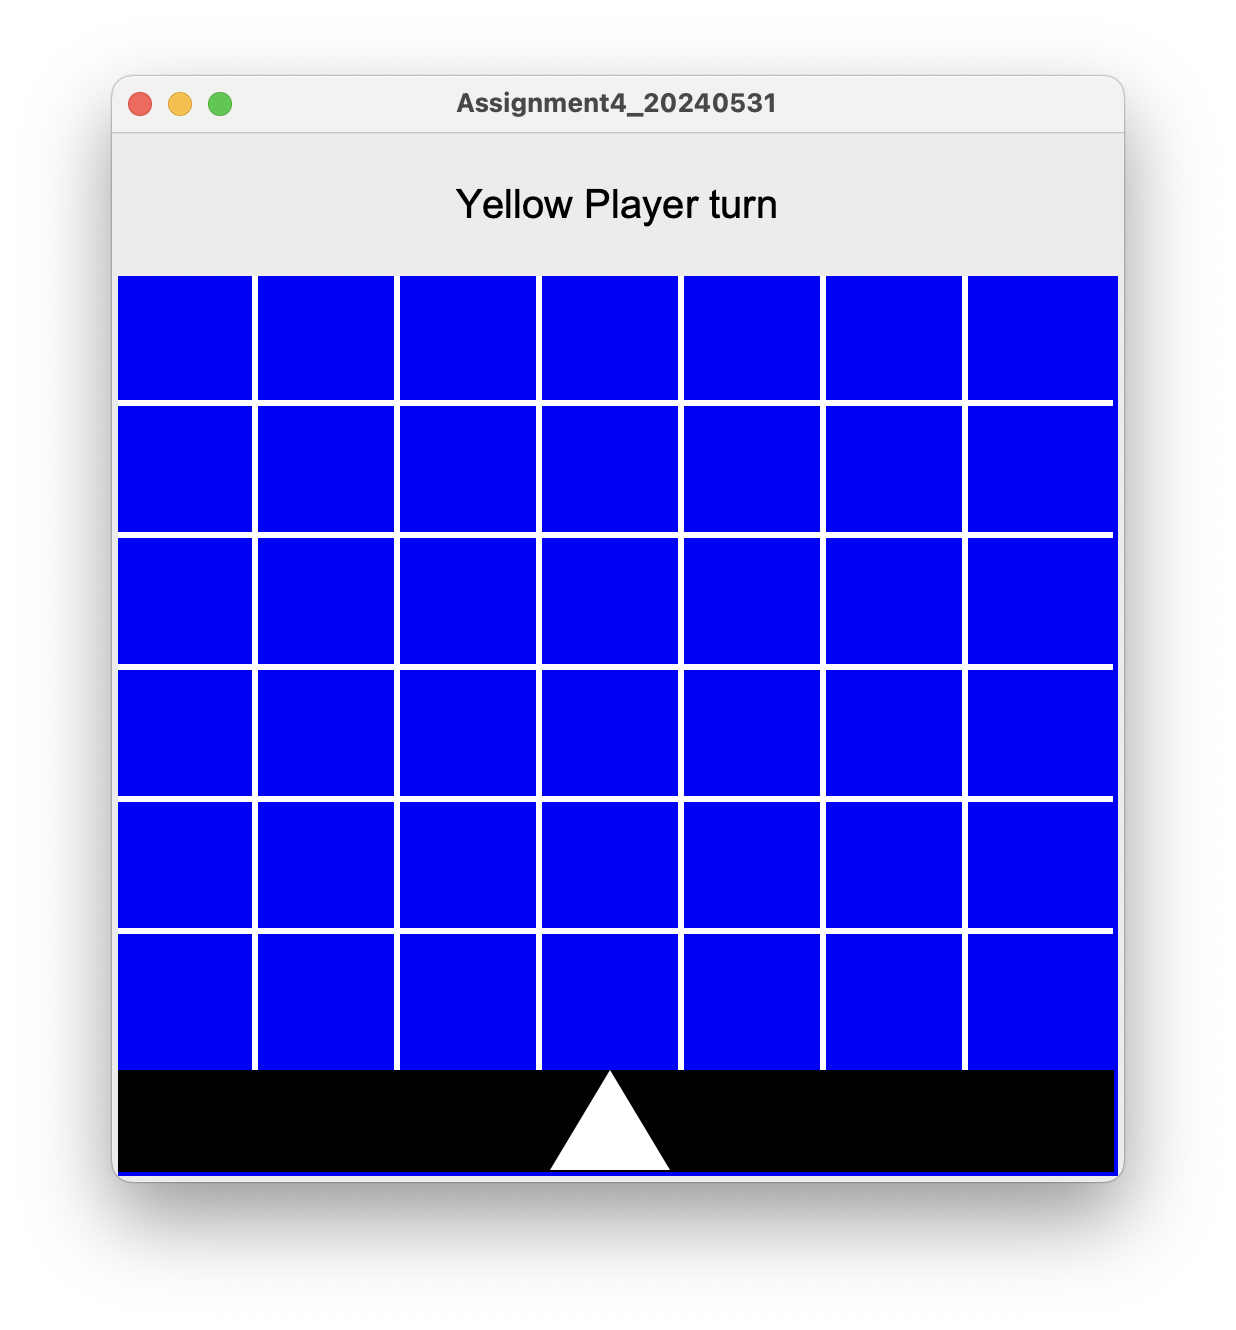
\includegraphics[width=6cm]{assets/screenshots/initial.png}
    \caption{실행 모습. 초기 화면}
    \label{img:1}
  \end{center}
\end{figure}
\begin{figure}
  \begin{center}
    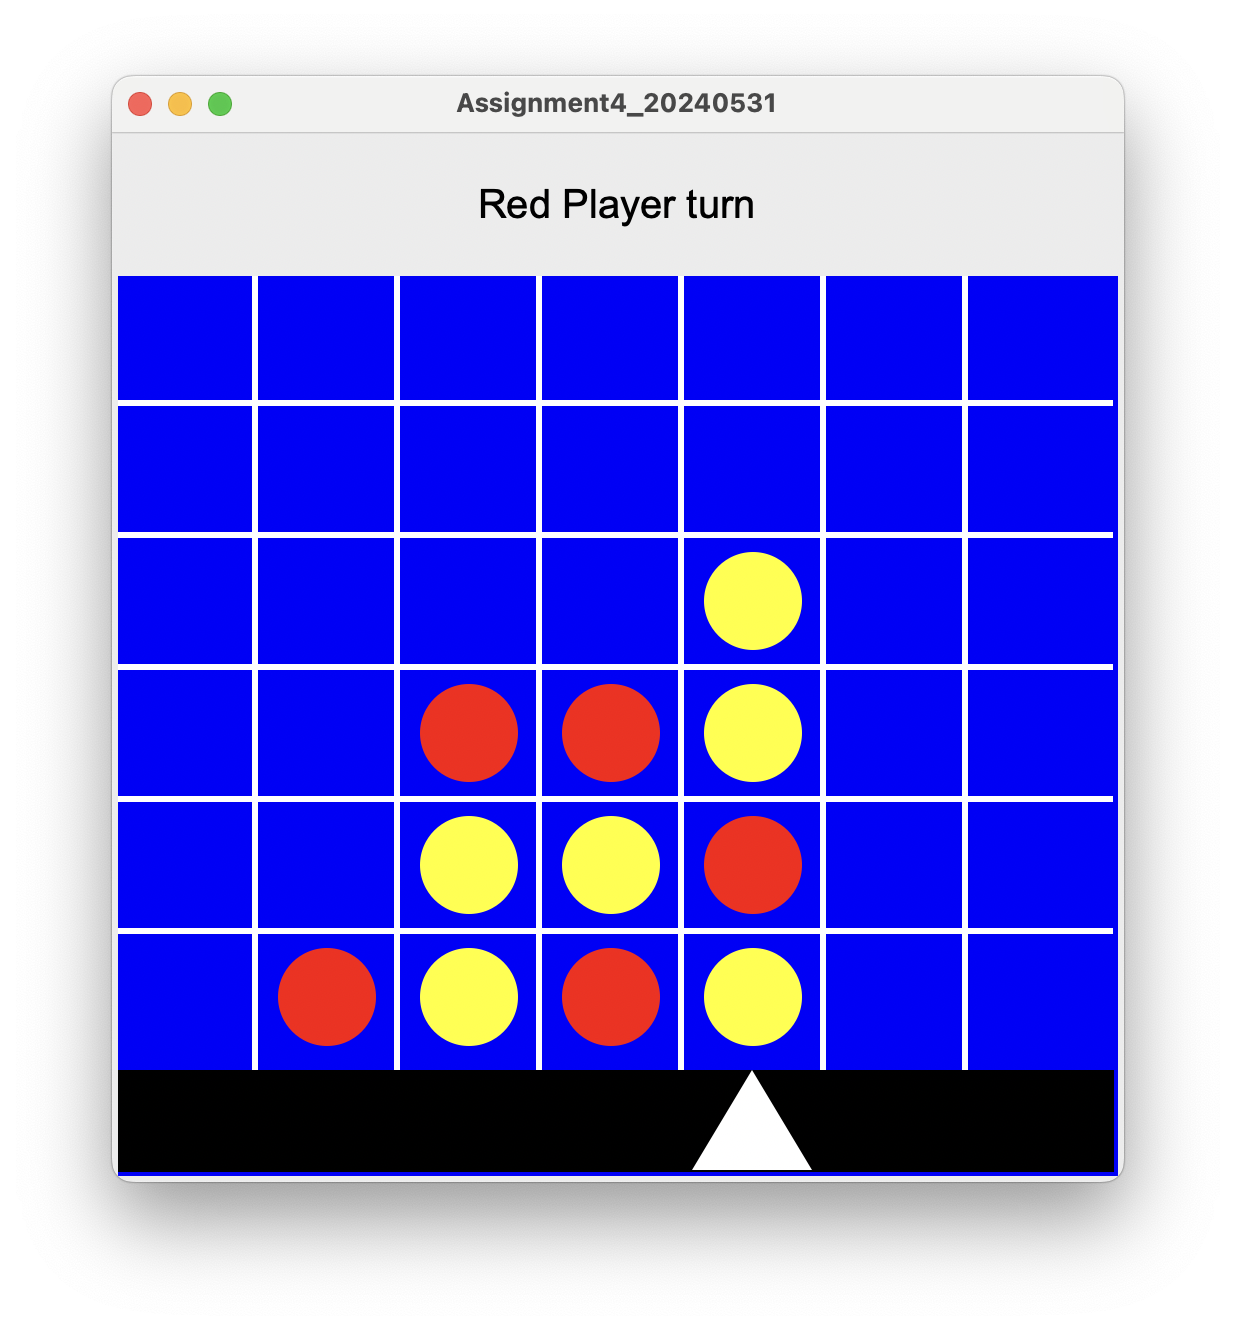
\includegraphics[width=6cm]{assets/screenshots/mid.png}
    \caption{실행 모습. 게임 중간 모습}
    \label{img:2}
  \end{center}
\end{figure}
\begin{figure}
  \begin{center}
    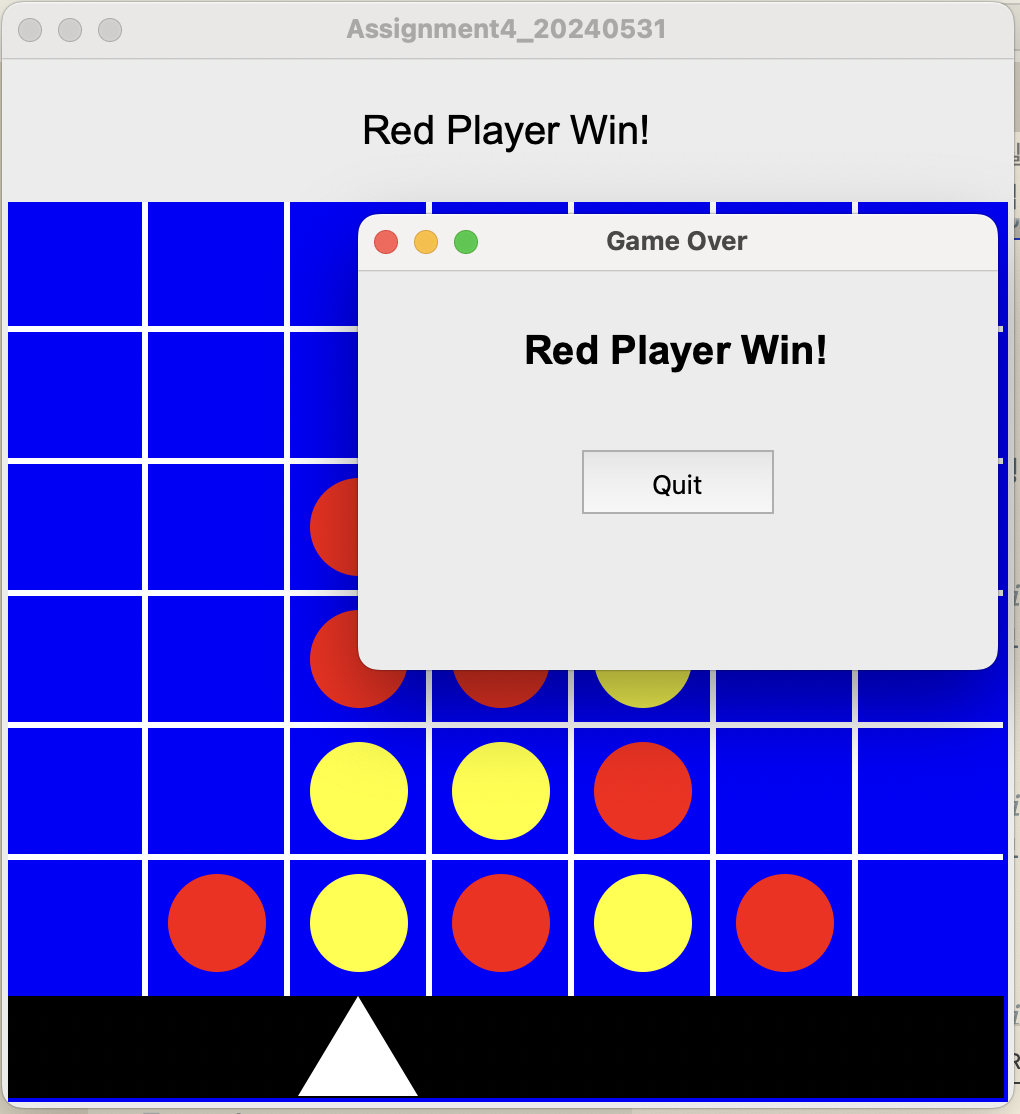
\includegraphics[width=5cm]{assets/screenshots/end.png}
    \caption{실행 모습. 게임 종료}
    \label{img:3}
  \end{center}
\end{figure}
\begin{figure}
  \begin{center}
    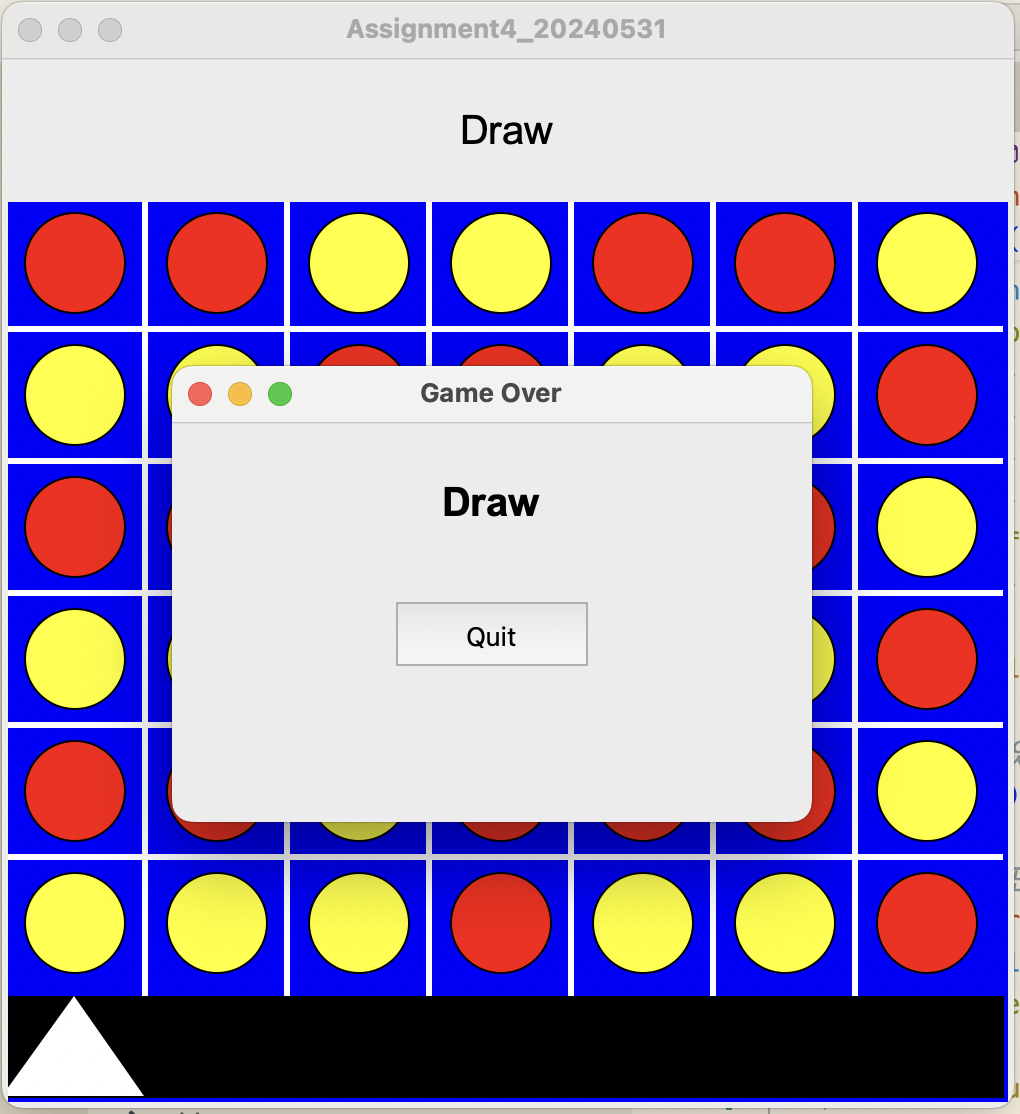
\includegraphics[width=5cm]{assets/screenshots/draw1.png}
    \caption{실행 모습. 게임 종료 (무승부)}
    \label{img:4}
  \end{center}
\end{figure}

\begin{itemize}
  \item 그림 \ref{img:1}\은 실행 직후 초기 모습이다. 문제 파일의 요구사항대로 프로그램 제목 및 게임판, 기타 UI를 표현하고 있다. 상단 문구 ('Yellow Player turn')을 통해 Yellow Player의 차례임을 알 수 있다.
  \item 그림 \ref{img:2}\은 게임 진행 중간 모습으로, 번갈아 가며 공을 착수하고 있다. 현재 Red Player 턴으로 화면 상단에 'Red Player turn' 문구가 출력되고 있다.
  \item 그림 \ref{img:3}\은 게임 종료 모습으로, Red Player가 승리한 모습이다.
  \item 그림 \ref{img:4}\은 무승부로 게임이 종료된 모습이다.
\end{itemize}

\section{토론}

\subsection{Info.update 메소드 (명세 추가)}

게임 화면의 플레이어 정보를 업데이트하기 위해서는 Info 인스턴스의 변수
중 label 변수에 접근해 옵선을 바꾸어야 한다. 이를 단순화하기 위해서
Info.update 메소드를 정의해 사용했다.

이 메소드는 표시할 문구를 인자로 받으며, 이 문구대로 플레이어 정보 표시 문구를 수정하는 일을 한다.

\subsection{Board.\_\_init\_\_ 메소드 (명세 변경)}

Board class 내부에서 root 인스턴스와 info 인스턴드에 접근해야 할 일이 있었다.
플레이어 정보 문구를 수정하거나, 게임 종료 창을 생성할 때 각각 info 인스턴스와 root 인스턴스가 필요하다.

이를 위해 Board.\_\_init\_\_ 생성자의 인자를 수정하여 root와 info를 받도록 만들었고,
함수 내부에서 self.root와 self.info에 인스턴스를 저장해두었다가 나중에 필요할 때 사용하도록 구현했다.

\section{결론}

파이썬과 Tkinter를 이용하여 Connect Four 게임을 만들어봄으로써 GUI 프로그램 만드는 방법을 익혔다.
다양한 위젯 사용, 클릭 및 마우스 이동 이벤트 처리 등을 익히며 GUI 프로그래밍에 익숙해질 수 있었다.
또한 객체 지향 프로그래밍에도 더 익숙해질 수 있었다.

\section{개선 방향}

승부 결정을 판단할 때, 현재는 모든 영역에서 4개의 공이 연속되었는지 확인하도록 코드를 작성했다.
하지만 이전에 착수했던 공들의 위치는 변하지 않으므로 이 곳에서 연속된 공이 나오지 않을 것임이 보장되고, 이 영역을 다시 확인하는 것은 불필요하다.
그러므로 마지막으로 착수한 공 주변에서만 연속된 공 4개가 등장하는지 판단하도록 개선하면 훨씬 효율적인 프로그램이 될 것이다.

\end{document}